\documentclass[a4paperm]{article}
%\documentclass[12pt,twocolumn]{article}

\usepackage[T2A]{fontenc}
\usepackage[utf8]{inputenc}
\usepackage[russian,english]{babel}
\usepackage{amsmath,amsthm,amssymb,stackrel}
\usepackage[affil-it]{authblk}
\usepackage{cite}
\usepackage{scrextend}
\usepackage{verbatim}
\usepackage{paralist}
\usepackage[mediumspace,mediumqspace,Grey,squaren]{SIunits}
\addtokomafont{labelinglabel}{\sffamily}
\usepackage{amsmath}
\usepackage{graphicx}
 \usepackage[usenames, dvipsnames]{color}
 \usepackage{multirow}
 \usepackage{longtable}
 \usepackage{lineno}
 
 \usepackage{xr}
 
 
%\usepackage[none]{hyphenat} %no nyphenation

\usepackage{SIunits}
\usepackage{miller}
\usepackage[version=3]{mhchem}

\usepackage{float} %H with figures

\setlength{\parindent}{5ex}

 \usepackage{newfloat} %For numbering of supplemmentary figures
 \DeclareFloatingEnvironment[name={Supplementary Figure}]{suppfigure}

\graphicspath{{figures/}}
\externaldocument{supplementary/smose_supp}


\begin{document}

%\linenumbers

\title{New crystal structures of the transition metall dichalcogenides}


\author[1,2]{Pavel N. Gavryushkin
   \thanks{Electronic address: \texttt{gavryushkin@igm.nsc.ru, p.gavryushkin@g.nsu.ru}; Corresponding author}}     
\author[1]{Nursultan Sagatov}
\author[3]{Zakhar I. Popov}

\affil[1]{Sobolev Institute of Geology and Mineralogy, Siberian Branch of Russian Academy of Sciences, prosp. acad. Koptyuga 3, 630090 Novosibirsk, Russian Federation}
\affil[2]{Novosibirsk State University, Pirogova 2, Novosibirsk 630090, Russian Federation}
\affil[3]{ИБХФ}

\date{}
\maketitle

%\linenumbers

\begin{abstract}
\end{abstract}

%%%%%%%%%%%%%%%%%%%%%%%%%%%%%%%%%%%%%
\section*{Introduction}
%%%%%%%%%%%%%%%%%%%%%%%%%%%%%%%%%%%%%
Trsnaition metall dichalcogenides (TMD) crystallise in four main structural types: type of CdI2 (further denoted as C),type of MoS2 (further denoted as W), type of pyrite and less frequent type of marcasite.
Fisrt two structural types are characterised by the layered structures with S-M-S sandwiches bonded by the weak Van-der-Waals bonds. 
The 2D layers attracts considerable attention due to their semiconducting, superconduting and magnetic properties.
In particular,2D layers of MoS2, WS2, MoSe2, WSe2, and MoTe2 have a direct band gap and can be used as transistors and due to strong spin-orbit coupling are prespective spintronics.

The top-layer of sulphur in the the sandwich of MoS2 was successfully changed on the layer of Se with formation of the so-called Janus SMoSe structure  \cite{lu2017}.
In the present work based on crystal structure prediction technique and common crystallchemical consideration we reveal new stable Janus structures of Mo, W and V and perform their extensive topological analysis.
The special paper will be devoted to the electronic properties of the found structures.


\subsubsection{Crystal structures of MCh2, M=Mo,W,Vm, Ch=S,Se}
At ambient conditions both MoS2, WS2, MoSe2, WSe2 crystallises in the arche-type molibdenite (MoS2) structure (W, 2H polytype).
In these structure atoms of chalcogenides form close-packed layers placed exacly one under another along c-axis.
TM atoms occupy center of trigonal prismatic cavities between the layers.
Different stacking of such a 2D layers produce different polytypes, but they are out of scope of the present work, where we consider only isolated 2D-layers.

If the layers of chalcogene atoms are shifted such that the top-layerd is placed in triangular holes fromed by the atoms of bottom-layer, the archetype CdI2 (C, 1T polytype) structure is formed. 
In this case, TM atoms are in octahedral coordination.

Considered compounds are not yet known in the form of bulk crystal with 1T structure 

V is different from W and Mo in that it does not produce dichalcogenides at ambient conditions or this compounds needs some additional factors for stabilisation.
VS2 compound is not known.
VSe2 is known in the form 2H structure with additional V adoms in the centers of empty trigonal prisms in between the sandwiches and composition Se2V1.005
V1.04Te2 has not-layered structure with isolated clusters.



%%%%%%%%%%%%%%%%%%%%%%%%%%%%%%%%%%%%%
		\section{Methods}

%%%%%%%%%%%%%%%%%%%%%%%%%%%%%%%%%%%%%


%%%%%%%%%%%%%%%%%%%%%%%%%%%%%%%%%%%%%
			\section{Results}
%%%%%%%%%%%%%%%%%%%%%%%%%%%%%%%%%%%%%

\subsection{Similarity and differences of H, T, fxt and fes structures}

\par{H and T structures}
Although H and T structures are charactersied by the different coordination polyhedrons, they are similar in the manner of interconnection of these polyhedrons.
H structure consists of trigonal prisms MoS6 (MoS3Se3 for Janus structures), and T structure – of the octahedra of the same composition (Figure{\ref1H1T}).
Each trigonal prism share all three vertical edges with the neighboring prisms and does not share any faces.
As the result each vertice [and each verical edge] of the trigonal prism is common for three prisms (Figure{\ref1H1T}).
Similarly in T structure, each octahedron share all edges inclined to the plane of sulphur atoms with neighbouring octahedra, and each vertice is common for three octahedra (Figure{\ref1H1T}).
Bond valence of Mo--S bond is nearly equal to +4/6 and there are necessary three such a bonds on the sulphur atom to compensate its negative charge of 2$^-$.
The interconnection through the edges but not faces provides the longer distance between high-chargeed Mo4+ ions, reducing the energy of Couloumb interaction.
Thus in full accordance with Pauling rules, the arrangement of trigonal prisms and octahedra corresponding to H and T structures is most energetically favourable (Table \ref{enth_t}), in full accordance with the well known Pauling rules \cite{pauling1929}.

\par{fxt and fes structures}
The topology of recently found fes and fxt structures principally is different from that of H structure in the manner trigonal prisms are connected not only through edges but also through the faces.
The whole structure can be constructued from the two edge-connected trigonal prisms (Figure \ref{2prism_oct}b).
As the result, the enthalpis of fxt and fes structures are higher than that of H structure.
However, as well as in H and T structures, each at sulphur are connected to three Mo atoms in fxt and fes structure, providing the mentioned local charge balance.
As we will show below the local charge balance is not the obligatory requirement for the dynamical stability of the structure.

H and T structures provide the most homogenic distribution of sulphur as we as Mo atoms. 
Both nets of the Mo atoms and and S atoms consists of the geometrically equal triangular loops.
Eadge-sharing interconnection of trigonal prsims realised in fxt and fes structure inevitably leads to the appearance of the cavities bigger than that in H and T structures. 
In fes structure the cavities are in the form of the slightly compressed cube (Figure \ref{fes_SMoSe}).
The volume of these cavities is almost two times large than the volume of the cavities in H structure (38.8 against 17.7 \AA$^3$).
In casse of fxt structure, the volume of hexagonal cavities (Figure \ref{fxt_SMoSe} is almost 8 times greater in comparison with H structure (137.8 against 17.7 \AA$^3$).
In contrast to trigonal prisms, the face-sharing of the rights octahedra seems to be problematic for quasi 2D structure, as it is results in deviation from the flat arrangement (Figure\ref{2prism_oct}b).
However, as it will be shown belown, the dynamically stable structures with face sharing deformed octahedra can also produced. 


\begin{figure}[H]
        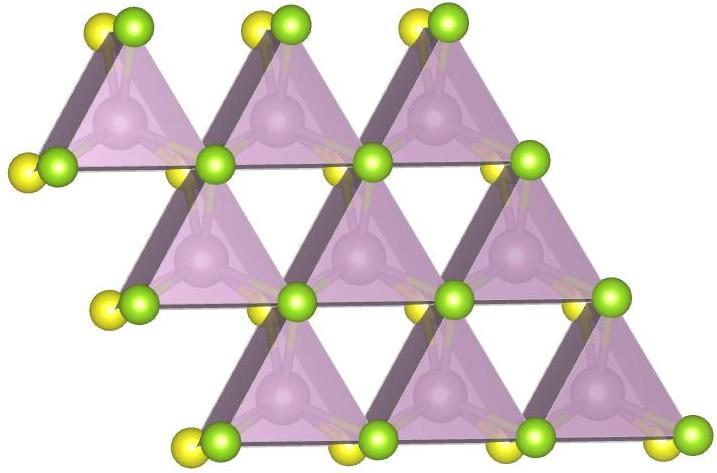
\includegraphics[width=0.45\textwidth]{1H.jpg}
        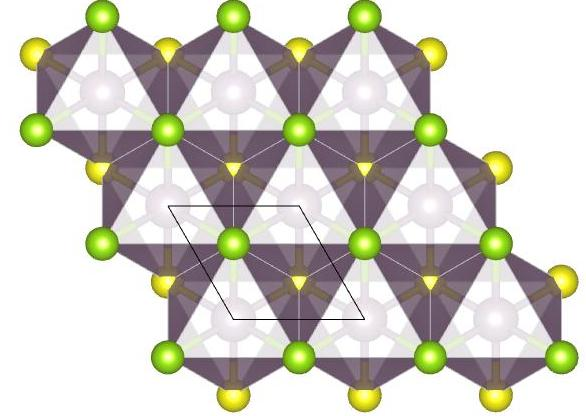
\includegraphics[width=0.45\textwidth]{1T.jpg}
        \caption{Packing of trigonal prisms and octahedra in H and T structures}
\label{1H1T}
\label{fes_fxt}
\end{figure}

\begin{figure}[H] \centering
	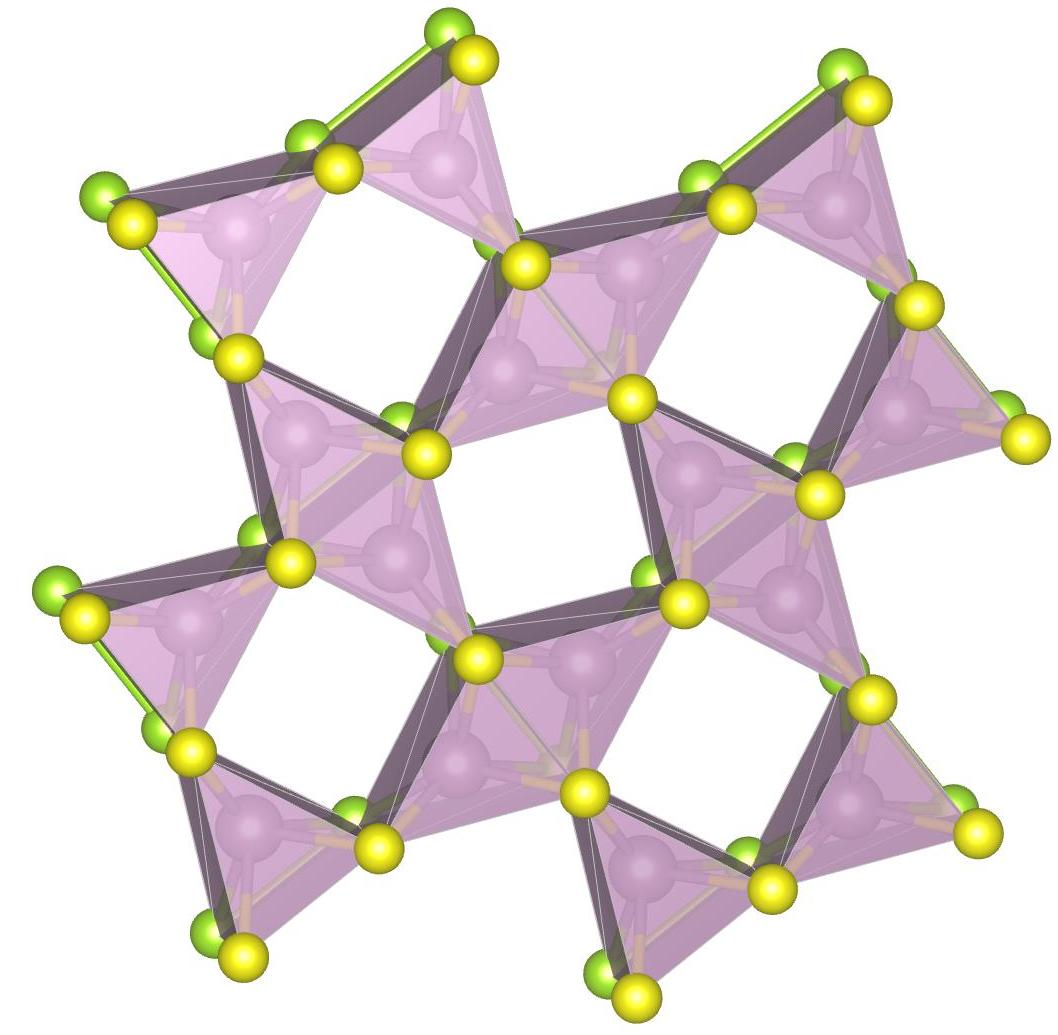
\includegraphics[width=0.5\textwidth]{fes_SMoSe.jpg}
        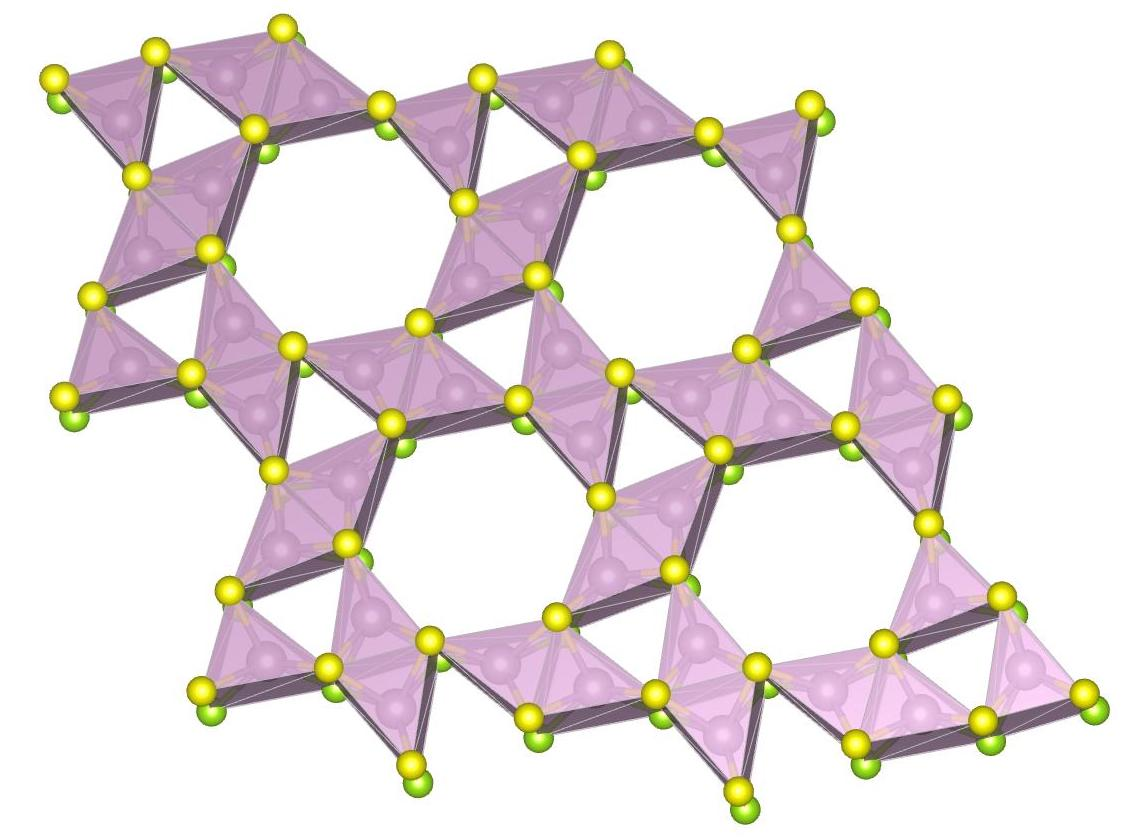
\includegraphics[width=0.5\textwidth]{fxt_SMoSe.jpg}
	\caption{Packing of trigonal prisms in fes and fxt structures.}
\label{fes_fxt}
\end{figure}

\begin{figure}[H] \centering
	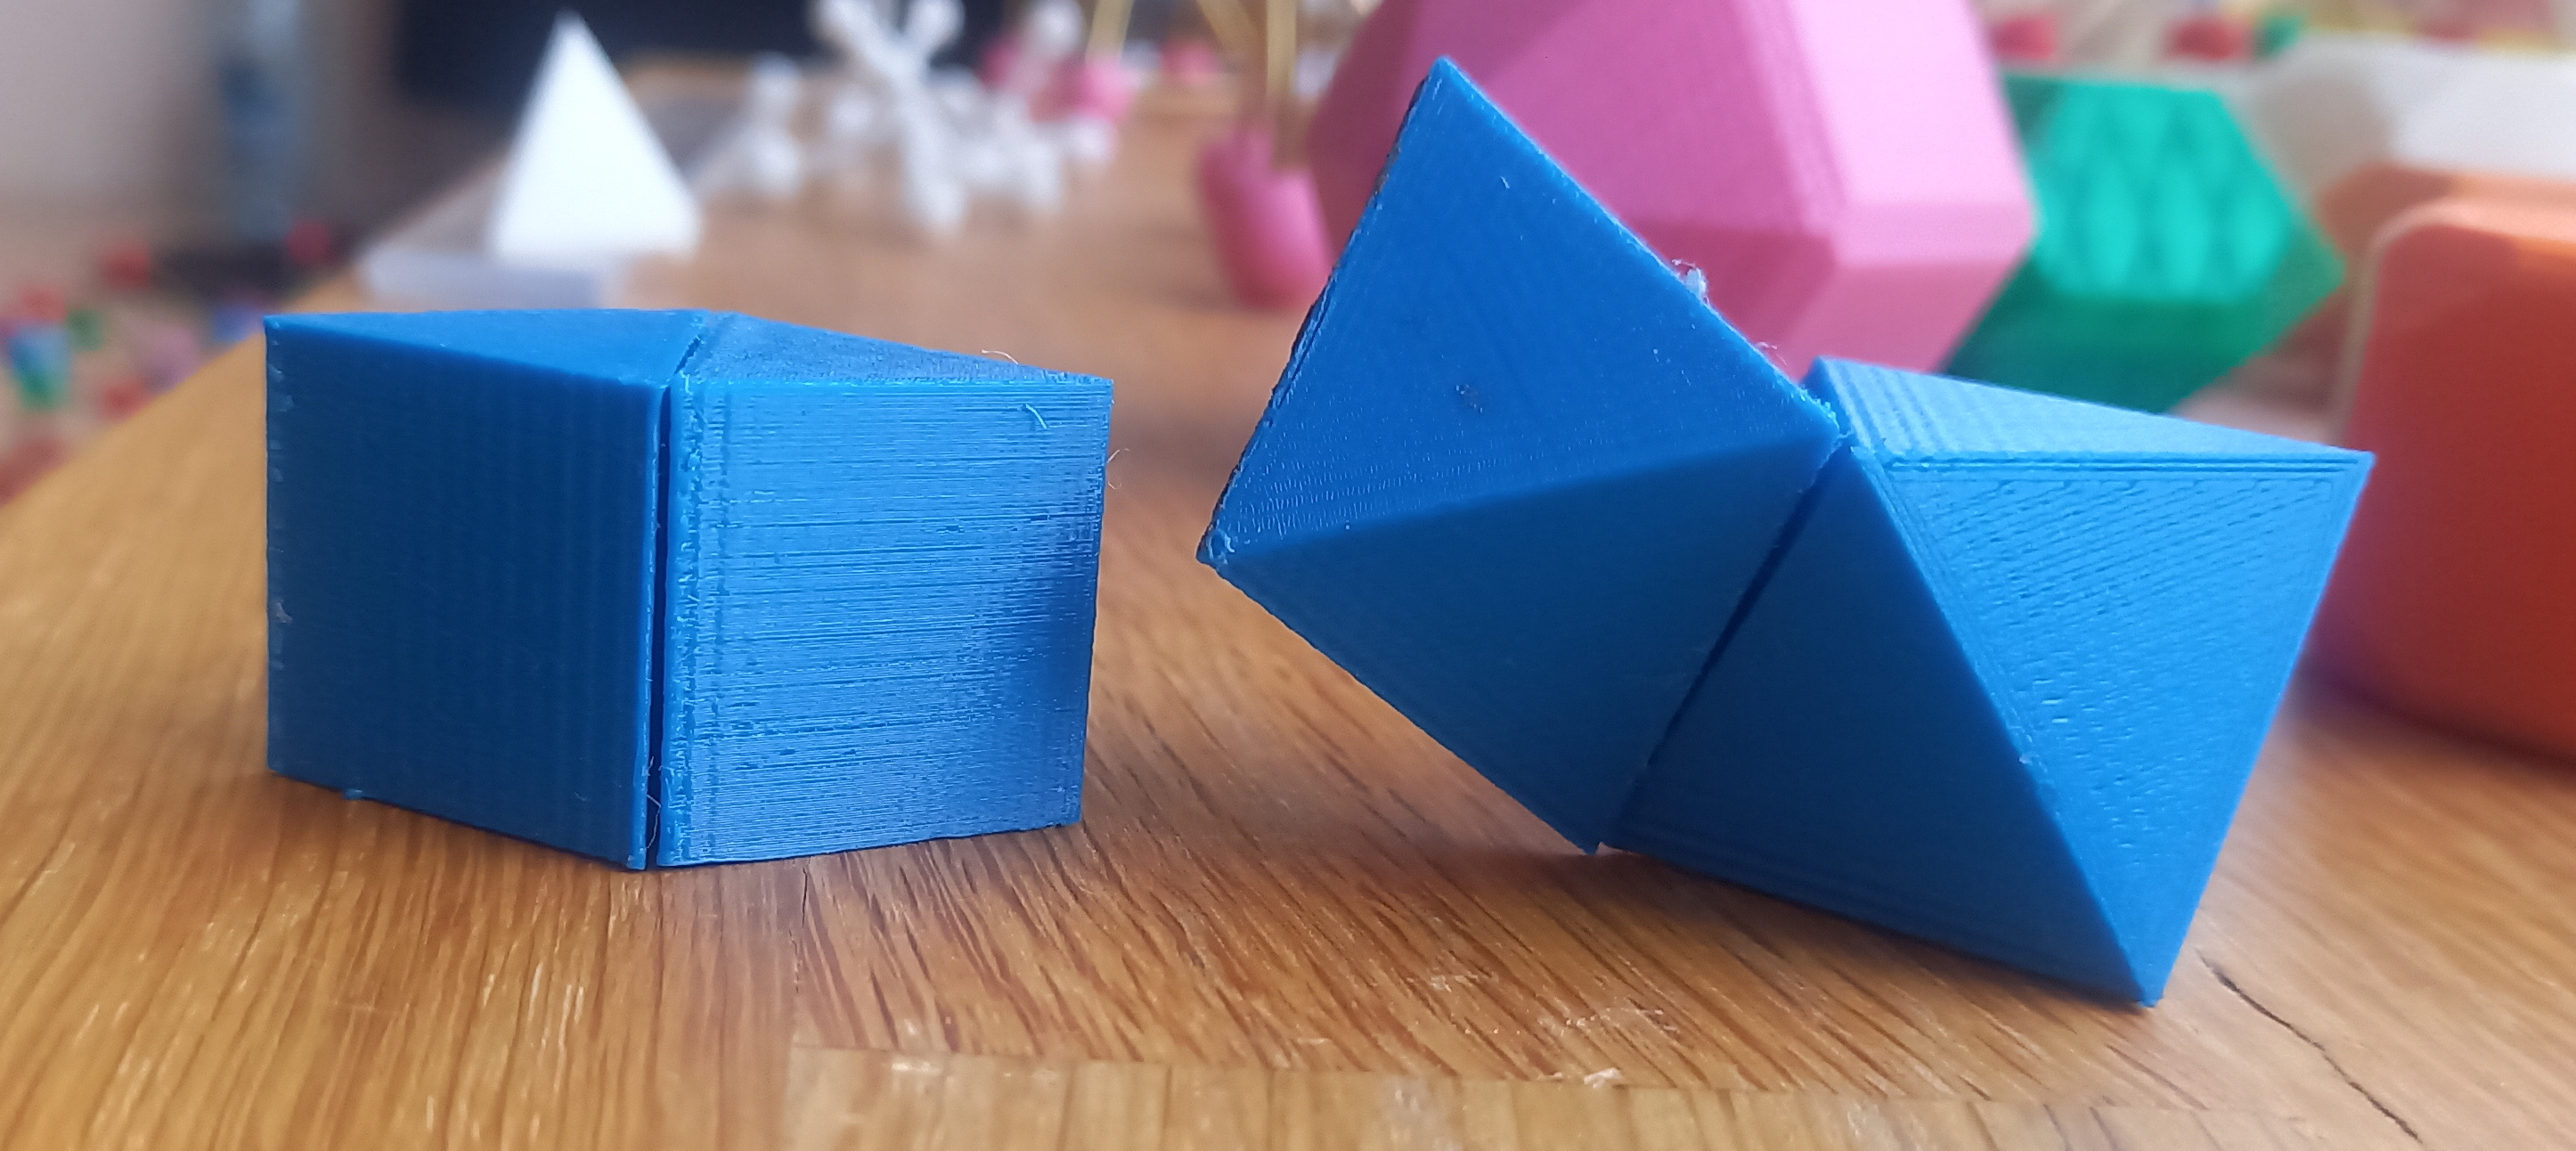
\includegraphics[width=0.5\textwidth]{2prism_oct.jpg}
	\caption{Two face-shared trigonal prisms and octahedra, the diviation from the horisontal plane in the last case is clearly visible}
\label{2prism_oct.jpg}
\end{figure}


%%%%%%%%%%%%%%%%%%%%%%%%%%%%%%%%%%%%%
		\subsection{The new crystal structures}
%%%%%%%%%%%%%%%%%%%%%%%%%%%%%%%%%%%%


%%%%%%%%%%%%%%%%%%%%%%%%%%%
\subsubsection{Structures with trigonal prismatic coordination}
%%%%%%%%%%%%%%%%%%%%%%%%%%

To compare topologies of H, fes, and fxt structures and produce similar structures with trigonal prismatic coordination, we present the structures as different fillings of the hexagonal net of sulphur atoms (Figure \ref{H-based}).
H-structure presents the most symmetric filling similar to chess-board with triagnular cells.
The fes structure can be also considered as the chess-board, but with doubled triangular cell, having the form of rhombuses.
After optimisation these rhombuses trasforms in the desribed above right squares.
In fxt structure the white loops are of two tipes.
The first are three doubled triangular (rhombuses) connected through the faces, having the form of right hexagons.
The second are primitive triangles.
The optimisation does not sufficiently change the form of the white loops, only slightly deforming hexagons.


Three new structures were produced by means of the filling of triangles in the hexagonal net of the sulphur atoms, named test1, test2, and test3.
We failed to produce new structures obeying the local charge balance, i.e. the structures in which each vertice of the trigonal prism is common for two other prisms.
In the structure test1, each sulphur atom is common for two or four filled prisms, in test2 and test 3 – for 2, 3, and 4 (Figure \ref{H-based}).
Test 3 structure is different from other structures in that it characterised by the presence of trigonal prisms with two common faces, while in all other structures prisms has no more than one common face.
This results in the shortening of the Mo--Mo--Mo distance, for Mo atoms placed in the neighbouring trigonal prisms.
Optimisation of test 3 structure sufficiently affect the arrangement of sulphur atoms coordinating these closely spaced Mo atoms, as we as atoms themselfes.
In the final structure the net of sulphur atoms is not the hexagonal one and corrdinations of some of Mo atoms, change from trigonal prsimatic to subsquare quadratic.

\begin{figure}[H] \centering
        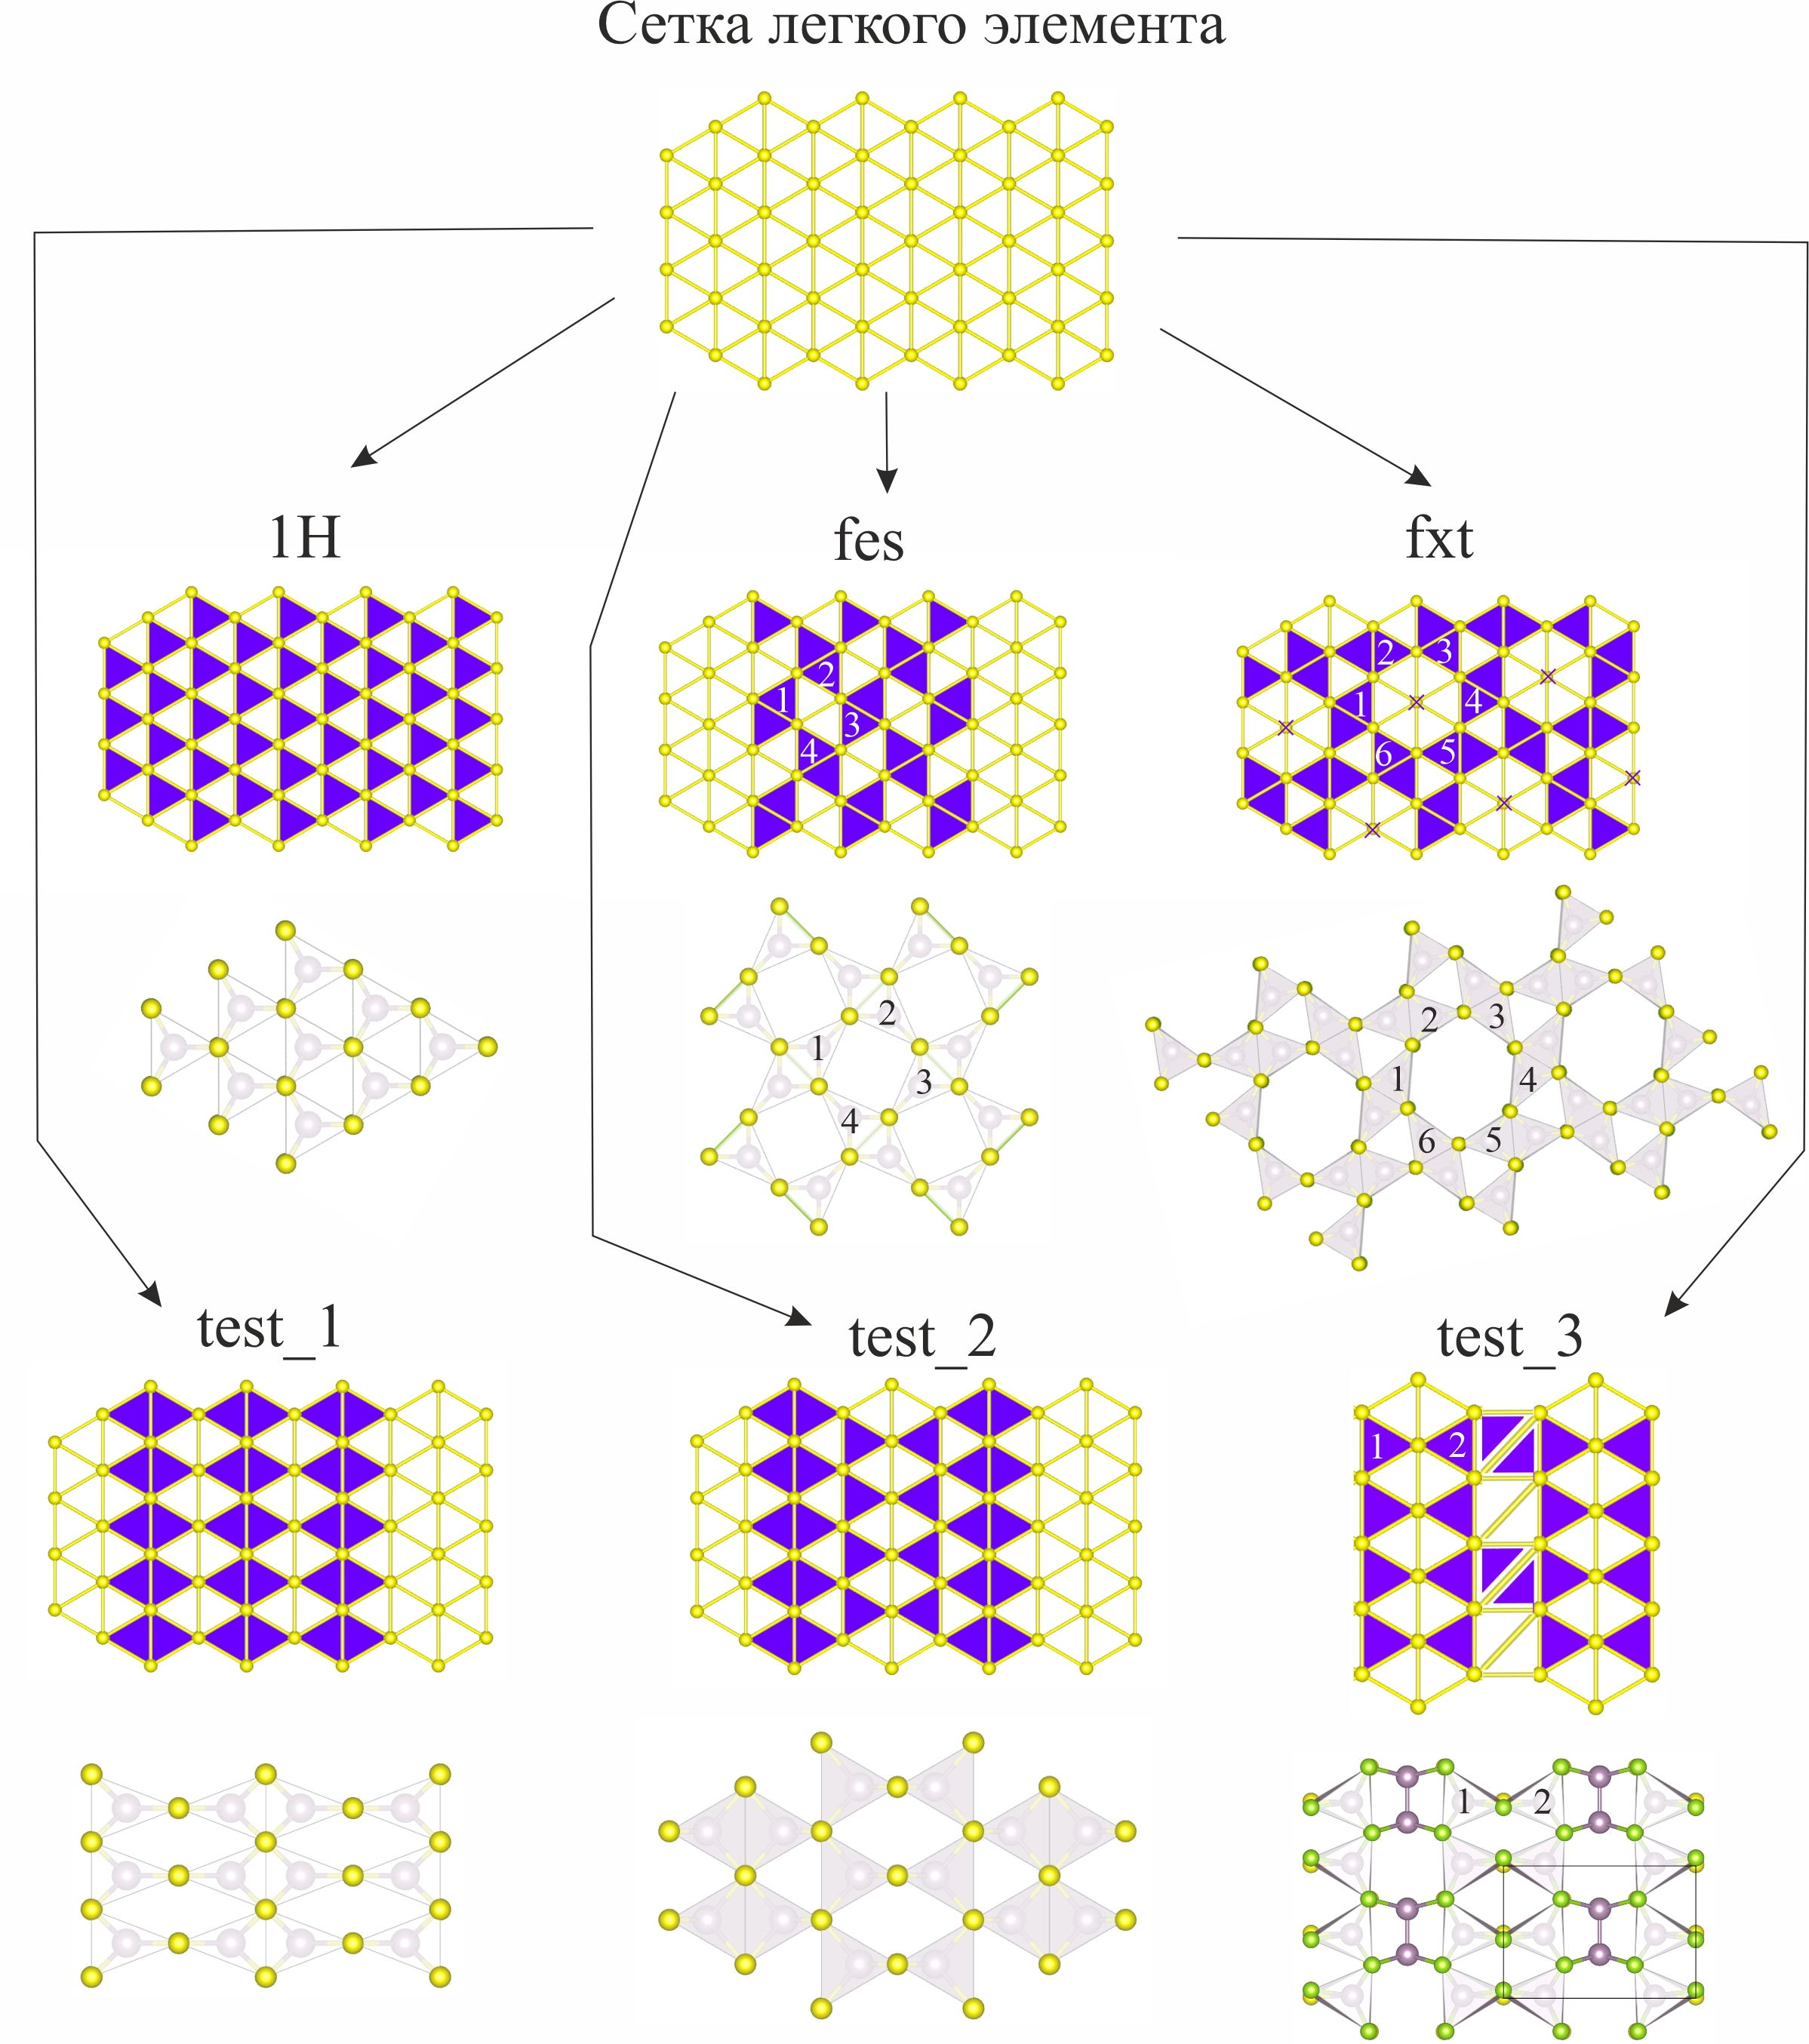
\includegraphics[width=0.8\textwidth]{H-based.jpg}
        \caption{The initial and optimised structures of MoSSe. Тут нужно убрать свзяь Mo-Mo для test3 и вомзможно показать Mo3 в профиль}
\label{H-based}
\end{figure}


Another structure chracterising by trigonal prismatic coordination was found by means of USPEX code.
It is sufficiently different from all the considered above structures in that three-fold axes of trigonal prisms are parallel to the place of sulphur atoms.
As the reuslt the loops of the net sulphur atoms is not more hexagonal, but square. 
This structure was colled Hhor (from H-horisontal)

%%%%%%%%%%%%%%%%%%%%%%%%
\subsubsection{Structures with octahedral coordination}
%%%%%%%%%%%%%%%%%%%%%%%

As it was mentioned above T structure, composed of closely packed octahedra does not give such a flexibility as H-structure, as contact of octahedra through the face results in the coorigation of the plane of sulphur atoms. 
One such a structure with face-shared octahedra have been found with AIRSS code.
In this structure each octahedra have four common edges and one common face.
The presence of the common face results in the sufficient corrugation of the layers of sulphur, in contrast to earlier considered structures, which a relatively flat ones.
This structure was called Thor.

\begin{figure}
	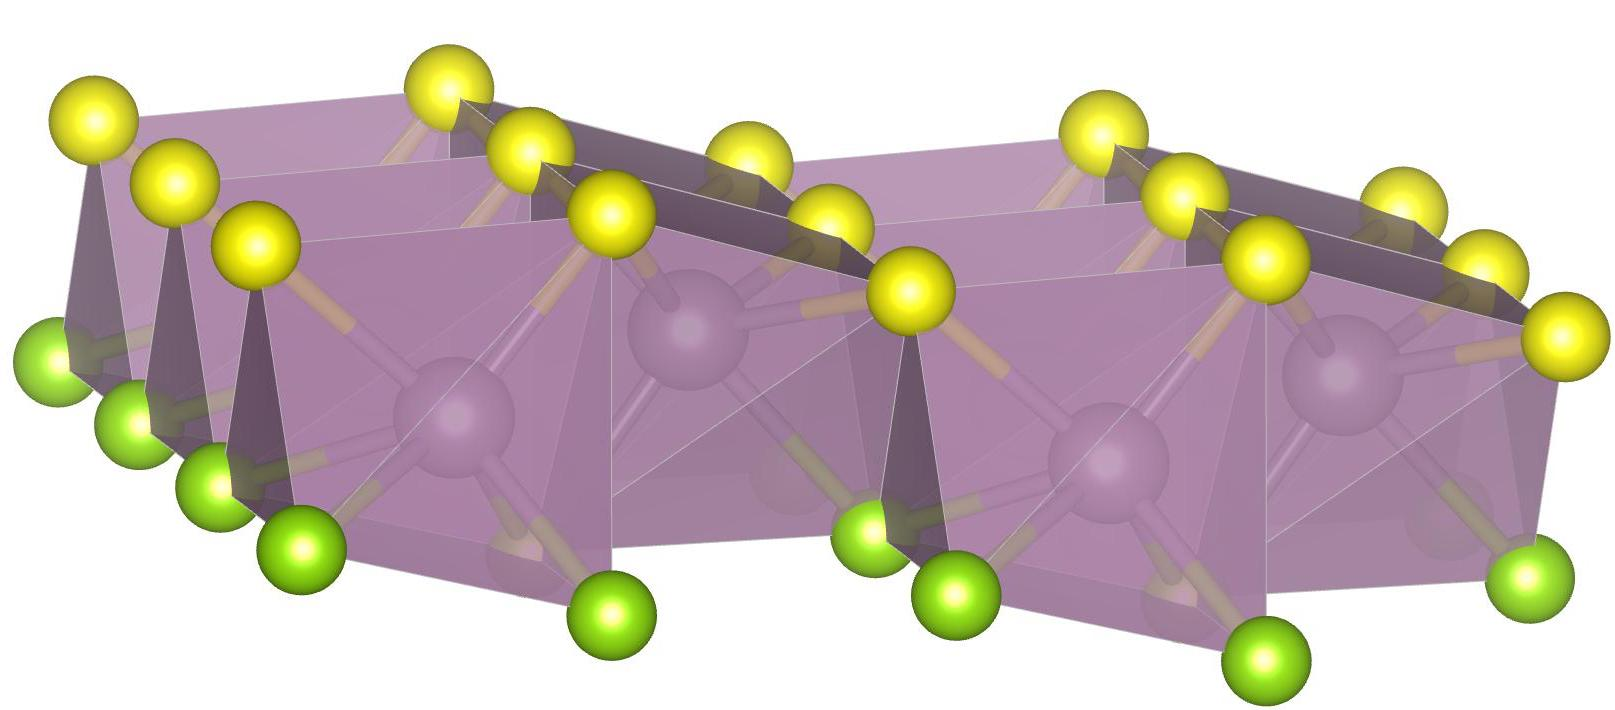
\includegraphics[width=0.45\textwidth]{H_hor_smose.jpg}
	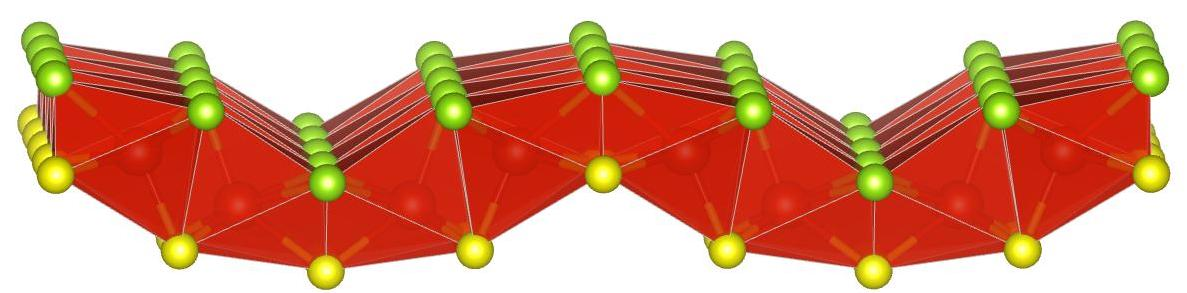
\includegraphics[width=0.45\textwidth]{T_hor_svse.jpg}
	\caption{Crystal sstructures with horis}
\label{hor_T_H}

\end{figure} 




\subsection{Stability of the predicted structures}




\end{document}


